\section{LED Brightness Control Using Potentiometer}

\subsection{Introduction}
A potentiometer is a variable resistor commonly used to provide
adjustable voltage in electronic circuits. In this experiment,
it is used as an analog input device that allows the user to control
the brightness of an LED. By rotating the potentiometer’s knob,
the voltage at its output (wiper) changes smoothly between 0V and
the supply voltage.

This varying voltage is read by the microcontroller through one of
its analog input pins. The microcontroller then maps the input value
to a range suitable for PWM (Pulse Width Modulation) output,
which is used to control the LED. A higher input voltage results
in a higher PWM duty cycle, making the LED appear brighter,
while a lower voltage dims it. This setup demonstrates how a simple
user interface element like a potentiometer can be used to control
an output device in real-time.



\subsection{Procedure}
1. Gathered an STM32F103C6 blue pill board, potentiometer, LED, $220\Omega$ resistor,
breadboard, and jumper wires.

2. Placed the potentiometer on the breadboard.
Connected the middle pin to PA0 (analog input), one side to 3.3V, and the other to GND.

3. Connected the LED's anode to PB0 (PWM output) through a $220\Omega$ 
resistor, and the cathode to GND.

4. Verified all connections were secure and correct.

5. Uploaded the code via PlatformIO. The LED brightness responded to the
potentiometer's wiper position.
\subsection{Diagram}
\begin{figure}[htbp]
    \centering
    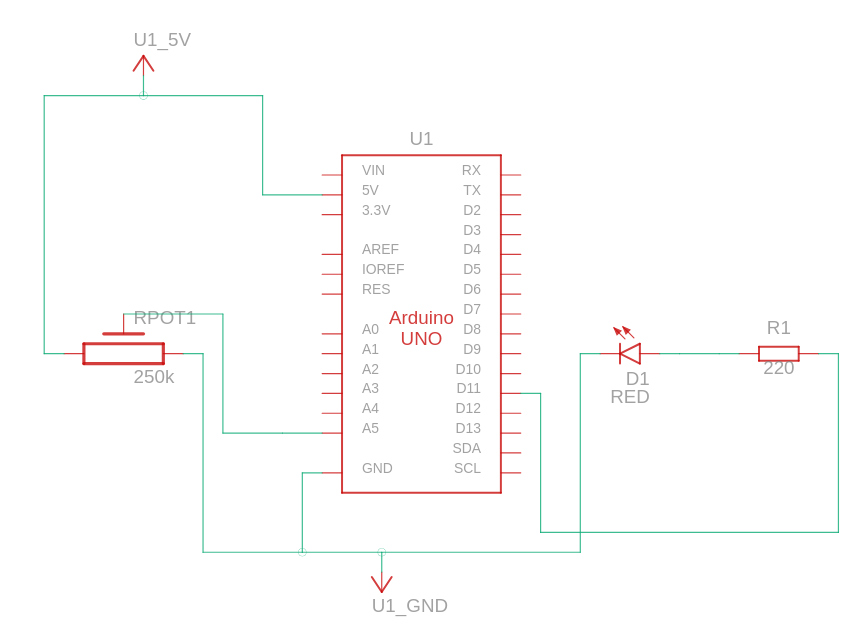
\includegraphics[width=0.6\textwidth]{img/pot.png}
    \caption{Schematic diagram of the circuit using Arduino in TinkerCAD}\label{fig:pott}
\end{figure}

\subsection{Source Code}
\begin{code}
\caption{Controlling LED brightness using potentiometer}
\begin{minted}[frame=single, linenos]{cpp}
#include <Arduino.h>
#define POT_PIN PA0
#define LED PB0
void setup() {
  pinMode(POT_PIN, INPUT);
  pinMode(LED, OUTPUT);
}

void loop() {
  int value = analogRead(POT_PIN);
  value = map(value, 0, 1023, 0, 255);
  analogWrite(LED, value);
  delay(500);
}
\end{minted}
    \label{code:Potentiometer}
\end{code}


\subsection{Discussion}

In this experiment, I successfully used a potentiometer to control
the brightness of an LED through PWM using an STM32 microcontroller
and the Arduino framework. The code read the analog voltage
from the potentiometer, mapped it to a 0–255 range, and used analogWrite() 
to adjust the LED's brightness accordingly.
As expected, turning the potentiometer smoothly increased 
or decreased the brightness, confirming that the analog input was
correctly processed and translated into a PWM output.

The results matched the intended behavior,
showing a clear and consistent change in LED brightness relative to
the potentiometer position. This demonstrated the effective use of
analog-to-digital conversion and pulse-width modulation in a microcontroller
environment.

Through this experiment, I learned how to read analog values from potentiometer,
map them for output control, and use PWM to vary LED intensity.
It also reinforced my understanding of basic circuit connections
and how software and hardware interact to produce real-time responses.

